\documentclass[a4paper, 12pt]{report}
\usepackage[utf8]{inputenc} % symboler, såsom æøå eller lignende
\usepackage{textcomp} % flere symboler, såsom €
\usepackage{fontawesome}
\usepackage{graphicx} % Muliggør brug af figurer
\usepackage{float} % Muliggør positionering af figurer
\usepackage{wrapfig} % Muliggør tekst og figur på samme linje
\usepackage{caption}
\usepackage{subcaption} % Muliggør subfigures
\usepackage{hyperref} % interaktive referencer!
\usepackage{csquotes} % bruges af babel pakken
\usepackage[english]{babel} % rapportens sprog. Skal også rettes i "main.tex" under "\selectlanguage"
\usepackage[font = small, labelfont = bf]{caption} % til mindre figur tekster hvor figur nummeret er fremhævet med fed
\usepackage{xcolor} % Til brugerdefinerede farvekoder
\usepackage{mathptmx} % Til brugerdefinerede font størrelser
\usepackage{pdfpages} % for an kunne importere hele pdf sider
\usepackage{booktabs} % for at definere /toprule og /midrule
\usepackage{hyperref} %Muliggør brug af hyperref

% load a colour package
\usepackage{xcolor}
\definecolor{aaublue}{RGB}{33,26,82}% dark blue
\usepackage{graphicx} % Set up how figure and table captions are displayed

\usepackage[font = small, labelfont = bf]{caption} % til mindre figur tekster hvor figur nummeret er fremhævet med fed
\usepackage{xcolor} % Til brugerdefinerede farvekoder
\usepackage{mathptmx} % Til brugerdefinerede font størrelser
\usepackage{pdfpages} % for an kunne importere hele pdf sider
\usepackage{booktabs} % for at definere /toprule og /midrule
\usepackage{ulem} %math
\usepackage{amsmath} %Math
\usepackage{xcolor,colortbl} % farver i tabeller
\usepackage{multicol}%kolonner
\hyphenpenalty=100000 % *EKSPERIMENTIEL* Forhindrer automatisk deling af ord

% ------ Marginer ------
\usepackage[left = 2cm, right = 2cm, bottom = 3cm ,top = 3.5cm]{geometry} % juster selv marginerne ved at indtaste andre tal

% ------ Farver ------
\definecolor{chapterNumColor}{RGB}{150, 150, 150} % 255, 255, 255 er helt hvid. 0, 0, 0 er helt sort

% ------ Lister ------
% ducomentation for list options: http://www.texnia.com/archive/enumitem.pdf
\usepackage{enumitem} % til redigering af lister
\setlist{itemsep = 0.5cm, itemindent = 0cm, labelsep = 0.5cm, leftmargin = 0.5cm} % globale indstillinger for lister.

% ------ Referencer ------
% Biblatex cheat sheet: http://tug.ctan.org/info/biblatex-cheatsheet/biblatex-cheatsheet.pdf
\usepackage[backend=biber, style=numeric, sorting=none]{biblatex}
\appto{\bibsetup}{\raggedright}
\addbibresource{referencer.bib} % fortæller hvad vores reference bibliotek hedder og hvor det er at finde i mappestrukturen


%\DeclareFieldFormat{postnote}{s. #1} % ændrer "page" til "s." i kilder ved enkelte sider
%\DeclareFieldFormat{multipostnote}{s. #1} % ændrer "pages" til "s." i kilder ved interval af sider

% Sørger for at der står et al. når der er flere end to forfattere.
\DefineBibliographyStrings{danish}{
  andothers = {et\addabbrvspace al\adddot}
}

% ------ Indholdsfortegnelse (Table of contents (TOC)) ------
\usepackage{tocloft}
\setcounter{secnumdepth}{3} % jo højere tallet er, jo "dybere" overskrifter bliver nummereret. 3 giver Chapter, section, subsection og subsubsection
\setcounter{tocdepth}{2} % dybden af indholdfortegnelsen. 1 viser chapter, section og sub
% \renewcommand{\cftpartleader}{\cftdotfill{\cftdotsep}} % prikker for parts
% \renewcommand{\cftchapleader}{\cftdotfill{\cftdotsep}} % prikker for chapters
% \renewcommand{\cftsecleader}{\hfill} % fjern prikker for sections
% \renewcommand{\cftsubsecleader}{\hfill} % prikker for subsections

% ------ Sidehoved og sidefod ------
\usepackage{lastpage} % Gør det muligt at få vist sidenummer for sidste side i rapporten.
\usepackage{fancyhdr} % Pakke til at modificere sidehoved og sidefod
\fancyhf{} % Sætter header og footer til ikke at indeholde noget - så vi er klar til at give det nyt indhold
\setlength{\headheight}{15pt} % Bestemmer hvor langt nede sidehovedet vises
\fancyfoot[R]{\thepage \ af \pageref{LastPage}} % Viser sidenummeret nederst til højre. Ændr "R" for at få det placeret et nyt sted
\fancyhead[L]{\leftmark} % placerer sidehoved indhold i øverste venstre side

\fancypagestyle{plain} % Brugerdefineret side når styletypen plain er valgt. I dette tilfælde er det hver gang et kapitel opstår. 
{
    \fancyhf{} % Sætter header og footer til ikke at indeholde noget - så vi er klar til at give det nyt indhold
    \renewcommand{\headrulewidth}{0pt} % Fjerner linjen øverst under sidehovedet
    \fancyfoot[R]{\thepage \ af \pageref{LastPage}} % Viser sidenummeret nederst til højre. Ændr "R" for at få det placeret et nyt sted
}
\pagestyle{fancy}

% ------ Style for kapitlers sidehoved ------
\usepackage{titlesec} % Til brugerdefinerede sidehoved
\titleformat{\chapter}{\fontsize{25pt}{25pt}\bfseries\color{black}}{{\color{chapterNumColor}\thechapter}}{15pt}{} % sætter fonttypen, skriftstørrelsen og farven på kapitel
\titlespacing*{\chapter}{0pt}{-50pt}{40pt} %Kapitelhøjde
\titleformat{\part}{\fontsize{40pt}{45pt}\bfseries\centering\color{black}}{{\color{chapterNumColor}\thepart}}{15pt}{}[\thispagestyle{empty}\addtocounter{page}{-1}] % sætter fonttypen, skriftstørrelsen og farven på parts

% ------ Selvlavede kommandoer til citater ------

\newcommand{\centerQuote}[3] % Indholdet i {} er navnet på den kommando der er lavet
{
    \begin{quote} % Sørger for at centrere dit citat
        \textit{"#1"} - \parencite[#2]{#3} % Laver formatet "Citat her" - (Efternavn, Årstal, s. sidetal)
    \end{quote} 
}

\newcommand{\inlineQuote}[3] % Indholdet i {} er navnet på den kommando der er lavet
{\textit{"#1"} \parencite[#2]{#3}} % Laver formatet "Citat her" - (Efternavn, Årstal, s. sidetal)

\usepackage{lipsum} % til at generere dummy text. Brug \lipsum[2] for at vise paragraf nr 2 i Lorem Ipsum. Brug \lipsum[4-7] for at vise paragraf 4 til 7 i Lorem Ipsum.

% ------ ToDo Notes ------
%ToDo Notes cheat sheet: https://mirrors.dotsrc.org/ctan/macros/latex/contrib/todonotes/todonotes.pdf
\setlength{\marginparwidth}{2cm} % Retter fejl med marginer i ToDo notes.
\usepackage{todonotes} % Muliggør brug af "ToDo notes" funktionalliteter

%------ Glossary ------
%Glossaries cheat sheet: https://mirrors.dotsrc.org/ctan/macros/latex/contrib/glossaries/glossariesbegin.pdf
\usepackage{glossaries} % Muliggør brug af "glossaries funktionen"
%\makenoidxglossaries % Muliggør udskift af glossary-list i dokumentet
\glstoctrue % Inkluderer glossary i toc
\input{glossary} % Muliggør brug af glossary.tex for samlede definitioner


%------ Boxes -------
\newlength{\mylen}
\settowidth{\mylen}{text to}


%------- Timelines -------
\usepackage{chronology}

%------- Til at lave culonner -----
\usepackage{multicol}

%------- Til at vise program code -----
\usepackage{inconsolata}
\usepackage{listings}
\lstset { %
    language=C++,
    basicstyle=\ttfamily\small,
    numberstyle=\footnotesize,
    numbers=left,
    backgroundcolor=\color{gray!10},
    frame=single,
    tabsize=2,
    rulecolor=\color{black!30},
    title=\lstname,
    escapeinside={\%*}{*)},
    breaklines=true,
    breakatwhitespace=true,
    framextopmargin=2pt,
    framexbottommargin=2pt,
	extendedchars=true,
    literate={å}{{\r{a}}}1 {ø}{{\o{}}}1 {á}{{\'a}}1 {ã}{{\~a}}1 {é}{{\'e}}1,
    %inputencoding=utf8
}

%------- Requirements table -------
\newcolumntype{L}[1]{>{\raggedright\let\newline\\\arraybackslash\hspace{0pt}}m{#1}}
\newcolumntype{C}[1]{>{\centering\let\newline\\\arraybackslash\hspace{0pt}}m{#1}}
\newcolumntype{R}[1]{>{\raggedleft\let\newline\\\arraybackslash\hspace{0pt}}m{#1}}
\usepackage{longtable, array}
% \setlength\extrarowheight{0pt}
% \setlength{\arrayrulewidth}{0.3mm}
\renewcommand{\arraystretch}{1.5}
\usepackage{makecell}
\usepackage{mwe}


% ------ Strike through text --------
\usepackage{soul}


%------- Bash color coding ----------
\lstset{ 
    language=bash, % choose the language of the code
    basicstyle=\fontfamily{pcr}\selectfont\footnotesize\color{black},
    keywordstyle=\color{black}\bfseries, % style for keywords
    numbers=left, % where to put the line-numbers
    numberstyle=\tiny, % the size of the fonts that are used for the line-numbers
    showspaces=false, % show spaces adding particular underscores
    showstringspaces=false, % underline spaces within strings
    showtabs=false, % show tabs within strings adding particular underscores
    frame=single, % adds a frame around the code
    tabsize=2, % sets default tabsize to 2 spaces
    rulesepcolor=\color{gray},
    rulecolor=\color{black},
    captionpos=b, % sets the caption-position to bottom
    breaklines=true, % sets automatic line breaking
    breakatwhitespace=false, 
    emph={rosrun,int,char,double,float,unsigned,void,bool},
    emphstyle={\color{blue!50}},
}

%---------- Ditto mark---------

\usepackage{tikz}
\newcommand{\dittotikz}{%
    \tikz{
        \draw [line width=0.12ex] (-0.2ex,0) -- +(0,0.8ex)
            (0.2ex,0) -- +(0,0.8ex);
        \draw [line width=0.08ex] (-0.6ex,0.4ex) -- +(-1.5em,0)
            (0.6ex,0.4ex) -- +(1.5em,0);
    }%
}

%----------- For having recurring text in the report to show the same ----------

\usepackage{clipboard}


\usepackage{multicol} % to insert columns
%%%%%%%%%%%%%%%%%%%%%%%%%%%%%%%%%%%%%%%%%%%%%%%%
% Macros for the title page
%%%%%%%%%%%%%%%%%%%%%%%%%%%%%%%%%%%%%%%%%%%%%%%%
%Creates the aau title page
\newcommand{\aautitlepage}[3]{%
  {
    %set up various length
    \ifx\titlepageleftcolumnwidth\undefined
      \newlength{\titlepageleftcolumnwidth}
      \newlength{\titlepagerightcolumnwidth}
    \fi
    \setlength{\titlepageleftcolumnwidth}{0.5\textwidth-\tabcolsep}
    \setlength{\titlepagerightcolumnwidth}{\textwidth-2\tabcolsep-\titlepageleftcolumnwidth}
    %create title page
    \thispagestyle{empty}
    \noindent%
    \begin{tabular}{@{}ll@{}}
      \parbox{\titlepageleftcolumnwidth}{
        \iflanguage{danish}{%
          \includegraphics[width=\titlepageleftcolumnwidth]{00 - Images/aau_logo_da.pdf}
        }{%
          
\includegraphics[width=\titlepageleftcolumnwidth]{00 - Images/aau_logo_en.pdf}
        }
      } &
      \parbox{\titlepagerightcolumnwidth}{\raggedleft\sf\small
        #2
      }\bigskip\\
       #1 & \\
    \end{tabular}
    \vfill
    \iflanguage{danish}{%
      \noindent{\footnotesize\emph{Rapportens indhold er frit tilgængeligt, men offentliggørelse (med kildeangivelse) må kun ske efter aftale med forfatterne.}}
    }{%
      \noindent{\footnotesize\emph{The content of this report is freely available, but publication (with reference) may only be pursued due to agreement with the author.}}
    }
    \clearpage
  }
}

%Create English project info
\newcommand{\englishprojectinfo}[8]{%
  \parbox[t]{\titlepageleftcolumnwidth}{
    \textbf{Title:}\\ #1\bigskip\par
    \textbf{Theme:}\\ #2\bigskip\par
    \textbf{Project Period:}\\ #3\bigskip\par
    \textbf{Project Group:}\\ #4\bigskip\par
    \textbf{Participant(s):}\\ #5\bigskip\par
    \textbf{Supervisor(s):}\\ #6\bigskip\par
    \textbf{Copies:} #7\bigskip\par
    \textbf{Page Numbers:} \pageref{LastPage}\bigskip\par
    \textbf{Date of Completion:}\\ #8
  }
}

%Create Danish project info
\newcommand{\danishprojectinfo}[8]{%
  \parbox[t]{\titlepageleftcolumnwidth}{
    \textbf{Titel:}\\ #1\bigskip\par
    \textbf{Tema:}\\ #2\bigskip\par
    \textbf{Projektperiode:}\\ #3\bigskip\par
    \textbf{Projektgruppe:}\\ #4\bigskip\par
    \textbf{Deltager(e):}\\ #5\bigskip\par
    \textbf{Vejleder(e):}\\ #6\bigskip\par
    \textbf{Oplagstal:} #7\bigskip\par
    \textbf{Sidetal:} \pageref{LastPage}\bigskip\par
    \textbf{Afleveringsdato:}\\ #8
  }
}


\begin{document}
%% FRONT MATTER
\fontfamily{ptm}\selectfont % times font
\pagenumbering{Roman} %use roman page numbering in the frontmatter

%  A simple AAU report template.
%  2015-05-08 v. 1.2.0
%  Copyright 2010-2015 by Jesper Kjær Nielsen <jkn@es.aau.dk>
%
%  This is free software: you can redistribute it and/or modify
%  it under the terms of the GNU General Public License as published by
%  the Free Software Foundation, either version 3 of the License, or
%  (at your option) any later version.
%
%  This is distributed in the hope that it will be useful,
%  but WITHOUT ANY WARRANTY; without even the implied warranty of
%  MERCHANTABILITY or FITNESS FOR A PARTICULAR PURPOSE.  See the
%  GNU General Public License for more details.
%
%  You can find the GNU General Public License at <http://www.gnu.org/licenses/>.
%
\pdfbookmark[0]{Front page}{label:frontpage}%
\begin{titlepage}
  \addtolength{\hoffset}{0.5\evensidemargin-0.5\oddsidemargin} %set equal margins on the frontpage - remove this line if you want default margins
  \noindent%
  \begin{tabular}{@{}p{\textwidth}@{}}
    \toprule[2pt]
    \midrule
    \vspace{0.2cm}
    \begin{center}
    \Huge{\textbf{
      Robot Programming Mini Project% insert your title here
    }}
    \end{center}
    \begin{center}
      \Large{
        - \Copy{Report title}{Showcase of programming abilities with ROS} -% insert your subtitle here
      }
    \end{center}
    \vspace{0.2cm}\\
    \midrule
    \toprule[2pt]
  \end{tabular}
  \vspace{4 cm}
  \begin{center}
    {\large
      Made by%Insert document type (e.g., Project Report)
    }\\
    \vspace{0.2cm}
    {\Large
      ROB1 B332-b%Insert your group name or real names here
    }
  \end{center}
  \vfill
  \begin{center}
  Aalborg University\\
    The Technological Faculty for IT and Design\\
    Department of Electronic Systems
  \end{center}
\end{titlepage}
\clearpage % forside

\cleardoublepage

\addcontentsline{toc}{chapter}{Title page}
\thispagestyle{empty}
\pdfbookmark[0]{English title page}{label:titlepage_en}
\aautitlepage{%
  \englishprojectinfo{
    \Paste{Report title} %title
  }{%
    ROS, C++, Programming %theme
  }{%
    1st Semester %project period
  }{%
    B332-b % project group
  }{%
    %list of group members
    Jesper Poscholann Hammer\\
    Maiken Cecilie Lanng\\
    Kjartan Nolsøe Jespersen\\ 
    Kasper Maarschalk Hytting
  }{%
    %list of supervisors
    %Matthias Rehm
  }{%
    1 % number of printed copies
  }{%
    \today % date of completion
  }%
}{%department and address
  \textbf{The Technological Faculty for IT and Design}\\
  Department of Electronic Systems\\
  Niels Jernes Vej 10, 9220 Aalborg Øst\\
  \href{http://www.aau.dk}{http://www.aau.dk}
}{% the abstract

}  % titelside (EN)
\chapter*{Preface\markboth{Preface}{Preface}}\label{ch:preface}
\addcontentsline{toc}{chapter}{Preface}
\thispagestyle{empty}

%This project has been interesting in the way that it taught me to work with ROS programming to the extent that I could see what Robotics Engineering is all about, peace out.
%\begin{flushright}
%- KNJ
%\end{flushright}


\vspace{\fill}

\textit{Signatures:}

\vspace{3\baselineskip}

\vspace{1mm}

\begin{minipage}[b]{0.45\textwidth}
 \centering
 \textbf{\large{x}}
 \rule{\textwidth}{0.5pt}\\
  {\footnotesize Jesper Poscholann Hammer}\\
 {\footnotesize jhamme19@student.aau.dk}
\end{minipage}
\hfill
\begin{minipage}[b]{0.45\textwidth}
 \centering
 \textbf{\large{x}}
 \rule{\textwidth}{0.5pt}\\
  {\footnotesize Maiken Cecilie Lanng}\\
 {\footnotesize mlanng19@student.aau.dk}
\end{minipage}
\vspace{3\baselineskip}

\vspace{1mm}

\begin{minipage}[b]{0.45\textwidth}
 \centering
 \textbf{\large{x}}
 \rule{\textwidth}{0.5pt}\\
  {\footnotesize Kjartan Nolsøe Jespersen}\\
 {\footnotesize knje20@student.aau.dk}
\end{minipage}
\hfill
\begin{minipage}[b]{0.45\textwidth}
 \centering
 \textbf{\large{x}}
 \rule{\textwidth}{0.5pt}
 {\footnotesize Kasper Maarschalk Hytting}\\
 {\footnotesize khytti19@student.aau.dk}
\end{minipage}

    
\newpage
\selectlanguage{english} %Skal også rettes i "preample.tex" under "\usepackage[danish, english]"
%%%%%

%% Contents
\tableofcontents
\thispagestyle{empty}
\cleardoublepage
%\listoftodos
%%%%%

%% MAIN MATTER
\pagestyle{fancy}
\pagenumbering{arabic} %use arabic page numbering in the mainmatter
%%%%%

%% INPUT HERUNDER
%\input{RPro-Mini-Project-B332b/02 - Sections/00-Agenda}
%\includepdf[pages=-,pagecommand={},width=\textwidth]{RPro-Mini-Project-B332b/03 - Notes/22-12-2020.pdf}
\chapter{Description of mini-project concept}

Seeing how our semester project was a demining robot, it only seemed fitting for us to make a mining-robot for this mini-project - this robot does however not lay landmines, it mines minerals.\\
\\
The basic idea was to make something similar to a computer game, so we took the tile-based movement known from especially turn-based role-playing games (RPGs) and mixed in the time\footnote{Turn 90 \textdegree = 30 sec. Turn 180 \textdegree = 50 sec. Move one tile forward = 45 sec. Move two tiles forward = 80 sec. Move one tile backward = 55 sec. Mine one unit of mineral = 60 sec. Check if cart is full = 10 sec. Unload cart = 70 sec.} aspect of real-time strategy games. The result was a mining robot that the user could command to perform simple tasks in a fictive mine.

\begin{figure}[!ht]
  \centering
  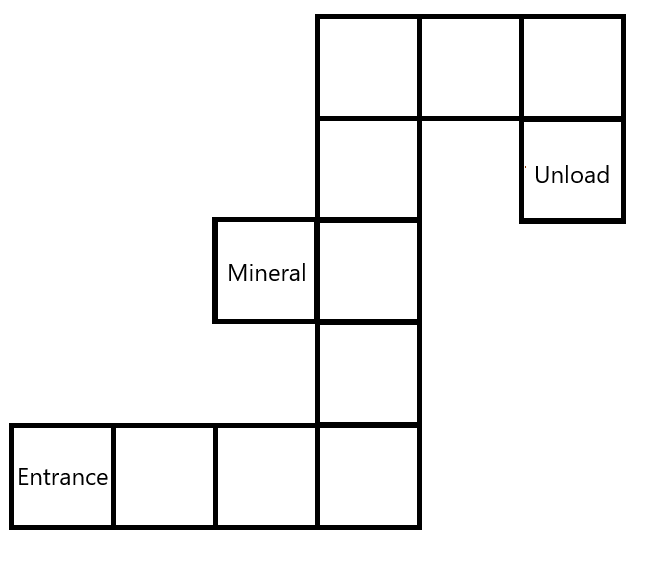
\includegraphics[width=6cm]{RPro-Mini-Project-B332b/00 - Images/mineMap.png}
  \caption{Map of the fictive mine}
\end{figure}

The robot will perform the tasks as they are programmed and output progress and results to a subscriber node. This can be compared to the text display often found in RPGs, where the player can see a text output of what is happening on screen.\\
\\
This is obviously only a small snippet, but it could be seen as a demonstration of how a single element of a larger computer game would behave and communicate as well as being manipulated by the user.\\
\\
\chapter{Methods}

\iffalse
Description of necessary hardware and software components. The project should at least feature 2 ROS nodes that are in communication with each other. And it should implement at least two functions. Usage of actual robot hardware is optional in this mini project.

I have splitted this into two chapters, "methods" and "implementation".
\fi

\section{C++}

C++ is a general-purpose programming language that is based on the former, but still active, C language. C++ added more functionalities, such as object-oriented programming which is missing from C, and being based on C, also includes the C capabilities to code on a low-level environment \cite{c++}.

ROS has been designed to work alongside C++, plus other programming languages, such as Python and Java.

\section{Robotic Operation System (ROS)}

Can be described as a meta-operating system, also called middleware. It acts like an independent system between the operating that runs on the computer/laptop one is working on and lower level hardware \cite{ros_core_components}.

The core elements of ROS are three things:
\begin{enumerate}
\setlength{\itemsep}{0.05\baselineskip}
    \item Communications Infrastructure
    \item  Robot-Specific Features
    \item Tools
\end{enumerate}

Having a communication infrastructure, means that the behaviour of ROS has a setup like a network in computing. In network computing one has a router that is connected to the computers on the network and acts like the go between between computer-to-computer. In ROS it is called nodes and these nodes are programs talking with each other in network behaviour and ROS functions as the master, i.e. the router.

These nodes have functionalities of asking, or in ROS terms, subscribing, for data from other nodes and publishing data out to the network that other nodes can subscribe to.\\

ROS can also record data that runs through its network so one can analyse the data and behaviour at later time, also use this recordings and re-simulate the data.

The robot-specific feature libraries that help one generate results, or part of the results. These libraries can be mapping, localisation, pose estimate and navigation amongst others.\\

%ROS is open source, so features get added to the lists continuously.\\

Tools that come with the ROS can help while building up the program(s). Rviz can be used for simulation, testing out the behaviour of the robot and its sensors in a virtual environment, and rqt for looking at the network of nodes running when we run our program(s) and look at the communication between the nodes \cite{ros_core_components}.

\subsection{ROS Publisher}

\iffalse
  /**
   * The advertise() function is how you tell ROS that you want to
   * publish on a given topic name. This invokes a call to the ROS
   * master node, which keeps a registry of who is publishing and who
   * is subscribing. After this advertise() call is made, the master
   * node will notify anyone who is trying to subscribe to this topic name,
   * and they will in turn negotiate a peer-to-peer connection with this
   * node.  advertise() returns a Publisher object which allows you to
   * publish messages on that topic through a call to publish().  Once
   * all copies of the returned Publisher object are destroyed, the topic
   * will be automatically unadvertised.
   *
   * The second parameter to advertise() is the size of the message queue
   * used for publishing messages.  If messages are published more quickly
   * than we can send them, the number here specifies how many messages to
   * buffer up before throwing some away.
   */
   
    /**
    * The publish() function is how you send messages. The parameter
    * is the message object. The type of this object must agree with the type
    * given as a template parameter to the advertise<>() call, as was done
    * in the constructor above.
    */
    
    Tell the master that we are going to be publishing a message of type std\_msgs/String on the topic chatter. This lets the master tell any nodes listening on chatter that we are going to publish data on that topic. The second argument is the size of our publishing queue. In this case if we are publishing too quickly it will buffer up a maximum of 1000 messages before beginning to throw away old ones.

    NodeHandle::advertise() returns a ros::Publisher object, which serves two purposes: 1) it contains a publish() method that lets you publish messages onto the topic it was created with, and 2) when it goes out of scope, it will automatically unadvertise. 

\fi

With ROS Publishing function we send massages across the ROS. This is one of the simpler functions of communication in ROS, called Topics. %More advanced communication functions are Services or Actionlib.

\begin{lstlisting}
    ros::Publisher "object" = nh.advertise<"template">("topic", "queue");
\end{lstlisting}
\begin{itemize}
\setlength{\itemsep}{0.05\baselineskip}
    \item "object" - name of the object initialisation of the Publisher function 
    \item "template" - how the data inside the message object is structured.
    \item "topic"\\- topic name telling subscribers where to find this published data on the network of nodes handled by the master, router.
    \item "queue"\\- the amount of how many messages are stored of those that haven't been used, if newer messages are generated, and the queue is full, the oldest messages will be discarded, and the newest added on top.
\end{itemize}

\subsection{ROS Subscriber}

\iffalse
  /**
   * The subscribe() call is how you tell ROS that you want to receive messages
   * on a given topic.  This invokes a call to the ROS
   * master node, which keeps a registry of who is publishing and who
   * is subscribing.  Messages are passed to a callback function, here
   * called chatterCallback.  subscribe() returns a Subscriber object that you
   * must hold on to until you want to unsubscribe.  When all copies of the Subscriber
   * object go out of scope, this callback will automatically be unsubscribed from
   * this topic.
   *
   * The second parameter to the subscribe() function is the size of the message
   * queue.  If messages are arriving faster than they are being processed, this
   * is the number of messages that will be buffered up before beginning to throw
   * away the oldest ones.
   */
  ros::Subscriber sub = n.subscribe("chatter", 1000, chatterCallback);
  
\fi

With ROS Subscribing function we receive messages across the ROS. This is one of the simpler functions of communication in ROS, called Topics. %More advanced communication functions are Services or Actionlib.

\begin{lstlisting}
    ros::Subscriber "object" = n.subscribe("topic", "queue", "function");
\end{lstlisting}
\begin{itemize}
\setlength{\itemsep}{0.05\baselineskip}
    \item "object" - name of the object initialisation of the Subscriber function 
    \item "topic"\\- topic name, telling the ROS which published data the this subscriber wants to connect to and receive data from. 
    \item "queue"\\- the amount of how many messages are stored of those that haven't been used, if newer messages are generated, and the queue is full, the oldest messages will be discarded, and the newest added on top. 
    \item "function" - when a message is received, the message will be sent to a function for further processing.
\end{itemize}

\newpage

\subsection{ROS custom messages}
Custom messages are messages where the user has defined a specific content. The messages consist of a number of fields (lines) each containing a type and a name. The data can be accessed using \textit{messagename.field}.\\
\\
The message is created by making a text file with the \textit{.msg} extension which is the compiled using catkin. The .msg-file is compiled into a header containing a class where the members are the fields of the original .msg-file.\\
\\
The custom massages can contain a range of types such as various integer variants, bool, strings and arrays. For a complete list refer to ROS Wiki.\\
\\
Source: ROS Wiki\cite{ROS_msg}

\subsection{String builder}
In order to transmit text AND variable data from one node to the other it is necessary to create a string builder, since ROS custom messages will only accept std::string messages and a std::ostringstream variable is needed to store multiple strings and variables together.

Practically we did this by creating a ostringstream variable called \textit{stringBuilder} and inserting strings and variables into this as needed. Subsequently the string variable for publication (logVar) is set equal to the stringBuilders \textit{.str}-member function.\\
\\
\begin{lstlisting}
    std::ostringstream stringBuilder;
    std::string logVar:
    
    stringbuilder << string << var << anotherString << anotherVar;
    logVar = stringBuilder.str();
\end{lstlisting}

\subsection{Clearing the string}
Regularly string and ostringstream can be leared using their \textit{.clear}-member function. In ROS messages however there are no clear functions. This is solved be inserting the ASCII return carriage (\textit{\textbackslash r}) command at the end of each text line. This forces the publisher to write the next line of text at the beginning of the string contained in the message.

%\newpage

%\subsection{Clear screen through ROS}
%When building a text display using text from one node and printing it in another, it is sometimes useful to be able to clear the screen in the subscribing node.

%We solved this be creating an if-statement which reads \textit{"cls"} as a parameter that calls \textit{system("clear");}. This way we are able to send a simple string to the subscribing node telling it that we want the screen cleared.
%\begin{lstlisting}
%    if (logOut.comm == "cls")
%        {
%            system("clear");
%        }
%\end{lstlisting}
\chapter{Implementation}

\section{Publisher}
The ROS publisher publishes messages onto the ROS network of nodes for any subscriber to read. In the code this is handled as described below.\\
\\
\begin{lstlisting}
void printLog()
    {
        rpro_mini_project::logOutput log;

        log.comm = logVar;

        mine_pub.publish(log);

        ros::spinOnce;
    }     
\end{lstlisting}
The $logOutput$ class of the $rpro\_mini\_project$ namespace is instantiated as \textit{log}. Then the contents of the class member \textit{comm} are set equal to the contents of the \textit{logVar} string variable.

Next \textit{log} is passed as a parameter when the $mine\_pub.pubish$ function is called. $mine\_pub$ is described below. Lastly the class \textit{spinOnce} of the namespace \textit{ROS} is called. This causes ROS to run its functions once thus advertising the existence of a new message on the topic and pubishing the message.\\
\\
\begin{lstlisting}
    mine_pub = nh.advertise<rpro_mini_project::logOutput>("miningLog",10);
\end{lstlisting}
In $mine\_pub$ we have nodehandle.anvertise which advertises new messages onto the ROS network of nodes. In this case the message $rpro\_mini\_project::logOutput$ are advertised onto the topic \textit{miningLog} at 10Hz.

\newpage

\section{Subscriber}
The ROS subscriber subscribes to topics on the ROS network of nodes and reads any advertised messages. In the code this is handled as described below.\\
\\
\begin{lstlisting}
void printLog(const rpro_mini_project::logOutput& logOut) {
        if (logOut.comm == "cls")
            {
                system("clear");
            }
        else
        {
            std::cout << logOut.comm << std::endl;
        }
    }
\end{lstlisting}
The printLog function has a constant reference to $rpro\_mini\_project::logOutput$ which is instantiated as \textit{logOut}. When a message of the \textit{logOutput}-class is published in the \textit{miningLog}-topic the contents are passed through the if-statements.

If the content of the class-member \textit{comm} equals "cls" the \textit{system}-function is called with the parameter "clear" which clears the terminal window.

If \textit{comm} contains anything else, the contents are printed in the console.\\
\\
\begin{lstlisting}
mine_sub = nh.subscribe("miningLog", 1000, &MiningOutput::printLog, this);
\end{lstlisting}
In $mine\_sub$ we have nodehandle.subscribe which subscribes to new messages - in this case on the \textit{miningLog}-topic. The second parameter is the message queue - how many messages will be kept in memory if our system cannot keep up with the flow of messages. Next is the pointer to the class-member who handles incoming messages.
\chapter{Discussion}\label{discussion}
\setlength{\parindent}{0ex}

The project containing the mining cart system has been an experience where several decisions have been made regarding the C++ code and ROS interaction. Firstly, it was to add a namespace to the two nodes and construct classes containing methods for executing various functions. This has been done as an overall personal preference, but also because the raw code is a lot easier to navigate when structured like this. The object oriented approach brings modularity into the code, and future expansion would be less complicated with this structure, this "expansion" would be done by converting some of the current methods to header files and enabling usage across nodes and subtracting them into classes relative to their function, but still in a structured manner as the code progresses in size. 

\iffalse
A note to the above:
The object oriented approach adds modularity to the code which prevents monolith coding, thus enabling the ability to easily scale the code.
\fi


\vspace{2mm}

A second initial thought in the planning stage of the mining cart software was to make a custom message containing a string, this has been done since a custom message gives more control but also the fact that a message can be changed in its original structure, thus adding the ability to expand the software as needed or if needed.

\vspace{40mm}

{\let\clearpage\relax \chapter{Conclusion}}

This mini-project shows a demonstration of a simple ROS package with two nodes, that contains a separate publisher in the first node, which publishes a custom string message to a subscriber in the second node.

The main functionality of the two nodes is as described in \textit{\autoref{implementation}} and this implementation are in the project groups opinion concluded as a success with room and functionality for expansion as described in \textit{\autoref{discussion}}.


\chapter{Conclusion}

This mini project shows a demonstration of the ROS Message function.

\vspace{10mm}

%% Forslag KMH
This mini-project shows a demonstration of a simple ROS package with two nodes, that is separately containing a publisher in the first node, that is publishing a custom string message to a subscriber in the second node. The main functionality of the two nodes is as described in \textit{\autoref{implementation}} and this implementation are in the project groups opinion concluded as a success with room and functionality for expansion as described in \textit{\autoref{discussion}}.


\chapter{GitHub Repository}

The following repository contains both our latex files and our project source code, this is made this way due to the fact that we work with different LaTeX configurations and to keep our project files in one place.

\vspace{2mm}

The correct path to the exam ROS package is:

\vspace{2mm}

\textbf{../code/src/rpro-mini-project}

\vspace{8mm}

This is to be found on the following link which points to the rpro-mini-project "home" directory.

\vspace{4mm}

\href{https://github.com/RiceCurry2/rpro-mini-project.git}{https://github.com/RiceCurry2/rpro-mini-project.git}




%%%%%


%%Backend
\printbibliography[
heading=bibintoc,
title={Bibliografi}
]


%\printnoidxglossary[sort=letter,nonumberlist]

\input{appendices}
%%%%%

\end{document}